\chapter{Theoretical Foundations}

After a short introduction to the terminology of Big Data, this chapter will discuss
the main characteristics of Big Data Analytics Applications and introduces the concept of
stream processing, which is one of the main characteristics of the popular streaming
frameworks Apache Flink and Apache Kafka. The underlying concepts both of these systems
and how they're used in context of Big Data Analytics will be explained at the
end of this chapter.

\section{Big Data}

According to \cite{Marz15} the term “Big Data” is a misleading name since it implies that
pre-existing data is somehow small, which is not true, or that the only challenge is the
sheer size of data, which is just one one them among others. In reality, the term Big Data
applies to information that can’t be processed or analyzed using traditional processes or
tools.

In the past decade the amount of data being created is a subject of immense growth.
More than 30,000 gigabytes of data are generated every second, and the rate of data
creation is only accelerating.\cite{Marz15}. People create content like blog posts, tweets, social
network interactions, photos, servers continuously log messages, scientists create detailed
measurements, permanently.

\begin{figure}[H]
	\centering
	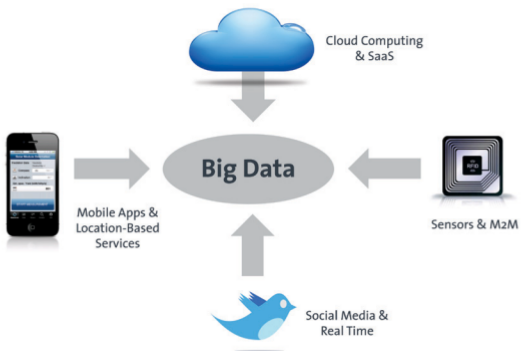
\includegraphics[width=0.7\textwidth]{../images/04-sources-of-bigdata.png}
	\caption{Sources of Big Data{\cite{Bitk12}}}
	\label{sources-of-bigdata}
\end{figure}

Through advances in communications technology, people and things are becoming in-
creasingly interconnected. Generally referred to as machine-to-machine (M2M), inter-
connectivity is responsible for double-digit year over year data growth rates. Finally,
because small integrated components are now affordable, it becomes possible to add
intelligence to almost everything. As an example, a simple railway car has hundreds
of sensors for tracking the state of individual parts and GPS-based data for shipment
tracking and logistics.\cite{Ziko12}

Besides the extremely growing amount of data, an increase in data diversity goes hand
in hand. It comes in its raw and unstructured, semistructured or structured form, which
makes processing it in a traditional relational system impractical or impossible.\cite{Bitk12}
describes, that around 85 percent of the data comes in an unstructured form, but containing
valuable information.

According to \cite{Marz15} \cite{Ziko12}, Big Data is defined by three characteristics:
\begin{description}
    \item [Volume] The amount of data present is growing because of growing amount of producers,
    e.g. environmental data, financial data, medical data, surveillance data.
    \item [Variety] Data varies in its form, it comes in different formats from different sources.
    \item [Velocity] Data needs to be evaluated and analyzed quickly, which leads to new challenges
    like analysis of large data sets with answers in seconds range, data processing in
    realtime, data generation and transmission at highspeed.
\end{description}
\begin{figure}[H]
	\centering
	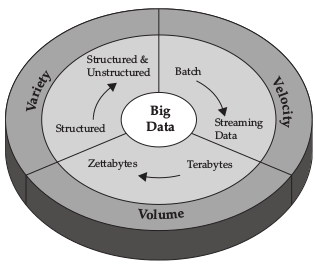
\includegraphics[width=0.7\textwidth]{../images/03-three-vs-of-bigdata.png}
	\caption{The three 'V's of Big Data{\cite{Ziko12}}}
	\label{three-vs-of-bigdata}
\end{figure}

A possible definition for Big Data could be derived as follows: \textit{Big Data refers to the use
of large amounts of data from multiple sources with a high processing speed for generating
valuable information based on the underlying data.}

\cite{Bitk12} proposes another characteristic as a fourth point called "Analytics", which will
be explained in the next section.

\section{Big Data Analytics Applications}

%Another definition comes from the the science historian George Dyson, who was cited by Tim O'Reilly in \cite{Dys13}:
%\textit{Big data is what happened when the cost of storing information became less than the cost of making the
%decision to throw it away.} It follows that the storage and extraction of valuable information from the immense amount of
%existing data has become the most important part of Big Data Analytics Applications.

Big Data Analytics describes the process of collecting, organizing and analyzing large
volumes of data with the aim to discover patterns, relationships and other useful informa-
tion extracted from incoming data streams \cite{Marz15}. The process of analytics is typically
performed using specialized software tools and applications for predictive analytics, data
mining, text mining, forecasting and data optimization.

The analytical methods raise data quality for unstructured data on a level that allows
more quantitative and qualitative analysis. With this structure it becomes posssible
to extract the data that is relevant by iteratively refined queries.

The areas of applications may be extremely diverse and ranges from analysis of financial
flows or traffic data, processing sensor data or environmental monitoring as explained in
the previous chapter.

The illustration below summarises the six-dimensional taxonomy \cite{Bitk14, Csa14} of Big
Data Analytics Applications.
\begin{figure}[H]
	\centering
	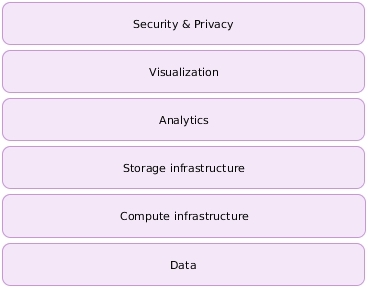
\includegraphics[width=0.7\textwidth]{../images/05-big-data-taxonomy.jpg}
	\caption{Taxonomy of Big Data Analytics Applications \cite{Bitk14, Csa14}}
	\label{taxonomy-bigdata-applications}
\end{figure}

The following section will discus the topic stream processing, which is part of the
"Compute infrastructure" layer shown in the figure above.

\section{Stream Processing}

Computing paradigms on big data currently differ at the first level of abstraction on
whether the processing will be done in batch mode, or in real-time/near real-time on
streaming data. This section is focussed on processing continous data streams in real-
time/near real-time and introduces Apache Flink and Apache Kafka as representants of
streaming frameworks.

According to \cite{Klepp16}, stream processing is the real-time processing of data continuously,
concurrently, and in a record-by-record fashion in which data is treated not as static tables
or files, but as a continuous infinite stream of data integrated from both live and historical
sources. It is needed, if “immediate” response to each event as it occurs is demanded by
the application. Various data streams could have own features. For example, a stream
from the financial market describes the whole data. In the same time, a stream for sensors
depends on sampling (e.g. get new data every 5 minutes).

The general approach is to have a small component that processes each of the events
separately. In order to speed up the processing, the stream may be subdivided, and the
computation distributed across clusters. Stream processing frameworks primarily addresses
parallelization of the computational load; an additional storage layer is needed to store
the results in order to be able to query them.

Benefits of stream processing:

\begin{itemize}
	\item Accessibility: live data can be used while still in motion, before being stored.
	\item Completeness: historical data can be streamed and integrated with live data for
	more context.
	\item High throughput: high-velocity and high-volume data can be processed with minimal latency.
\end{itemize}

In a formal way, a data stream is described as an ordered pair (S, T) where:
\begin{itemize}
	\item S is a sequence of tuples.
	\item T is a sequence of positive real time intervals.
\end{itemize}

It defines a data stream as a sequence of data objects, where the sequence in a data stream
is potentially unbounded, which means that data streams may be continuously generated
at any rate \cite{Nam15} and leads to the following characteristics:
\begin{itemize}
	\item the data arives continous
	\item the arrival of data is disorderen
	\item the size of the stream is potentially unbounded
\end{itemize}

After this short introduction to the basics of stream processing, the following sections
covers a short introduction of the streaming frameworks Apache Flink and Apache Kafka.
\subsection{Apache Flink}

As described in the documentation \cite{Flink16}, \textit{"Apache Flink is an open source platform for
distributed stream and batch data processing. Flink’s core is a streaming dataflow engine that
provides data distribution, communication, and fault tolerance for distributed computations over
data streams. Flink also builds batch processing on top of the streaming engine, overlaying native
iteration support, managed memory, and program optimization."}

The main components of Flink applications are formed by streams and transformations, in which
streams define intermediate results whereas transformations represent operations computed on one
or more input streams with one or more resulting streams.

The following code from \cite{Flink16} shows a basic Flink application, a working example of streaming
window word count application, that counts the words coming from a web socket in 5 second windows:


\begin{lstlisting}[caption={Basic Apache Flink streaming application}, captionpos=b, label={lst:basicflink}]
public static void main(String[] args) throws Exception {
        StreamExecutionEnvironment env = StreamExecutionEnvironment.getExecutionEnvironment();
        DataStream<Tuple2<String, Integer>> dataStream = env
                .socketTextStream("localhost", 9999)    (1)
                .flatMap(new Splitter())                (2)
                .keyBy(0)                               (2)
                .timeWindow(Time.seconds(5))            (2)
                .sum(1);                                (2)

        dataStream.print();                             (3)
        env.execute("Window WordCount");
    }

    public static class Splitter implements FlatMapFunction<String, Tuple2<String, Integer>> {
        @Override
        public void flatMap(String sentence, Collector<Tuple2<String, Integer>> out) throws Exception {
            for (String word: sentence.split(" ")) {
                out.collect(new Tuple2<String, Integer>(word, 1));
            }
        }
    }
\end{lstlisting}

On execution, Flink applications are mapped to streaming dataflows, consisting of streams
and transformation operators (3) where each dataflow starts with one or more sources (1)
the data is received from and ends in one or more sinks(3) the resulting stream is written
to.

The following overview summarises the most important streaming features of Apache Flink:

\begin{description}
    \item [Event time and out of order streams]
    Due to the distributed character of Big Data Analytics Applications, data doesn't arrive
    necessarily in the order that they are produced. Since version 0.10, Flink provides the
    concept of "event time", the processing of events by the time they happened in the real
    world to support "out of order" streams what enables consistently processing of events
    according to their timestamps.

    \item [Windows]
    Flink uses a concept called windows to divide a data stream that can be potentially infinite
    into finite slices based on the timestamps of elements or other criteria. This division
    is required when working with infinite streams of data and performing transformations that
    aggregate elements

    \item [Consistency, fault tolerance, and high availability]
    Flink guarantees consistent state updates and data movement in the presence of failures
    between selected sources and sinks. Such failures include machine hardware failures, network
    failures, transient program failures, etc. It supports worker and master failover,
    eliminating any single point of failure by providing  a checkpointing mechanism that recovers
    streaming jobs after failures.

    \item [Connectors and integration points]
    Flink integrates with a wide variety of open source systems for data input and output (Kafka,
    Elasticsearch and others) which makes technical decisions regarding the infrastructure quite flexible.
\end{description}

\subsection{Apache Kafka}

Apache Kafka is publish-subscribe messaging rethought as a distributed commit log. \cite{Kafka16}.
It is written in Scala and was initially developed at LinkedIn.

This excerpt from the paper \cite{Neha11} the team at LinkedIn published about Kafka describes the
basic principles:

\textit{A stream of messages of a particular type is defined by a topic. A producer can publish
messages to a topic. The published messages are then stored at a set of servers called brokers.
A consumer can subscribe to one or more topics from the brokers, and consume the subscribed
messages by pulling data from the brokers. (…) To subscribe to a topic, a consumer first creates
one or more message streams for the topic. The messages published to that topic will be evenly
distributed into these sub-streams. (…)  Unlike traditional iterators, the message stream iterator
never terminates. If there are currently no more messages to consume, the iterator blocks until
new messages are published to the topic.}

TODO: Role of Kafka as broker to ingest data


%\subsection{Related work}
%
%\subsubsection{Prometheus}
%
%\subsubsection{Datadog}
%
%\subsubsection{New Relic}
%
%\subsubsection{collectd}

%collectd is a daemon which collects system performance statistics periodically and
%provides mechanisms to store the values in a variety of ways, for example in RRD files.
%
%\subsubsection{collectd}
%
%StatsD is originally a simple daemon developed and  released by Etsy  to aggregate and summarize application metrics.
%With StatsD, applications are to be instrumented by developers using language-specific client libraries. These libraries
%will then communicate with the StatsD daemon using its dead-simple protocol, and the daemon will then generate aggregate
%metrics and relay them to virtually any graphing or monitoring backend.

\section{Summary}